\section{Проектирование программного средства}

\subsection{Разработка архитектуры программного средства}

После того, как были сформулированы функциональные требования к разрабатываемой
системе,  а  также  исходя  из  результатов  анализа  существующих
программных решений, можно определить основные моменты организации системы,  в
которой  будет  функционировать  разрабатываемое  программное  решение.

Процесс проектирования архитектуры программного обеспечения включает в себя сбор
требований, их анализ и создание проекта для компонента программного
обеспечения в соответствие с требованиями. Успешная разработка ПО должна
обеспечивать баланс неизбежных компромиссов вследствие противоречащих
требований;  соответствовать  принципам  проектирования  и  рекомендованным
методам,  выработанным  со  временем;  и  дополнять  современное оборудование,
сети и системы управления. 

Архитектуру  программного  обеспечения  можно рассматривать  как  сопоставление
между целью компонента ПО и сведениями о реализации в коде. Правильное понимание
архитектуры  обеспечит  оптимальный баланс требований и результатов. Только
программное обеспечение с хорошо продуманной архитектурой способно выполнять
указанные задачи с параметрами исходных требований, одновременно обеспечивая
максимально высокую производительность. Программное средство построено на основе
модульной архитектуры. 

\FloatBarrier
\begin{figure}[H]
\centering
	\fbox{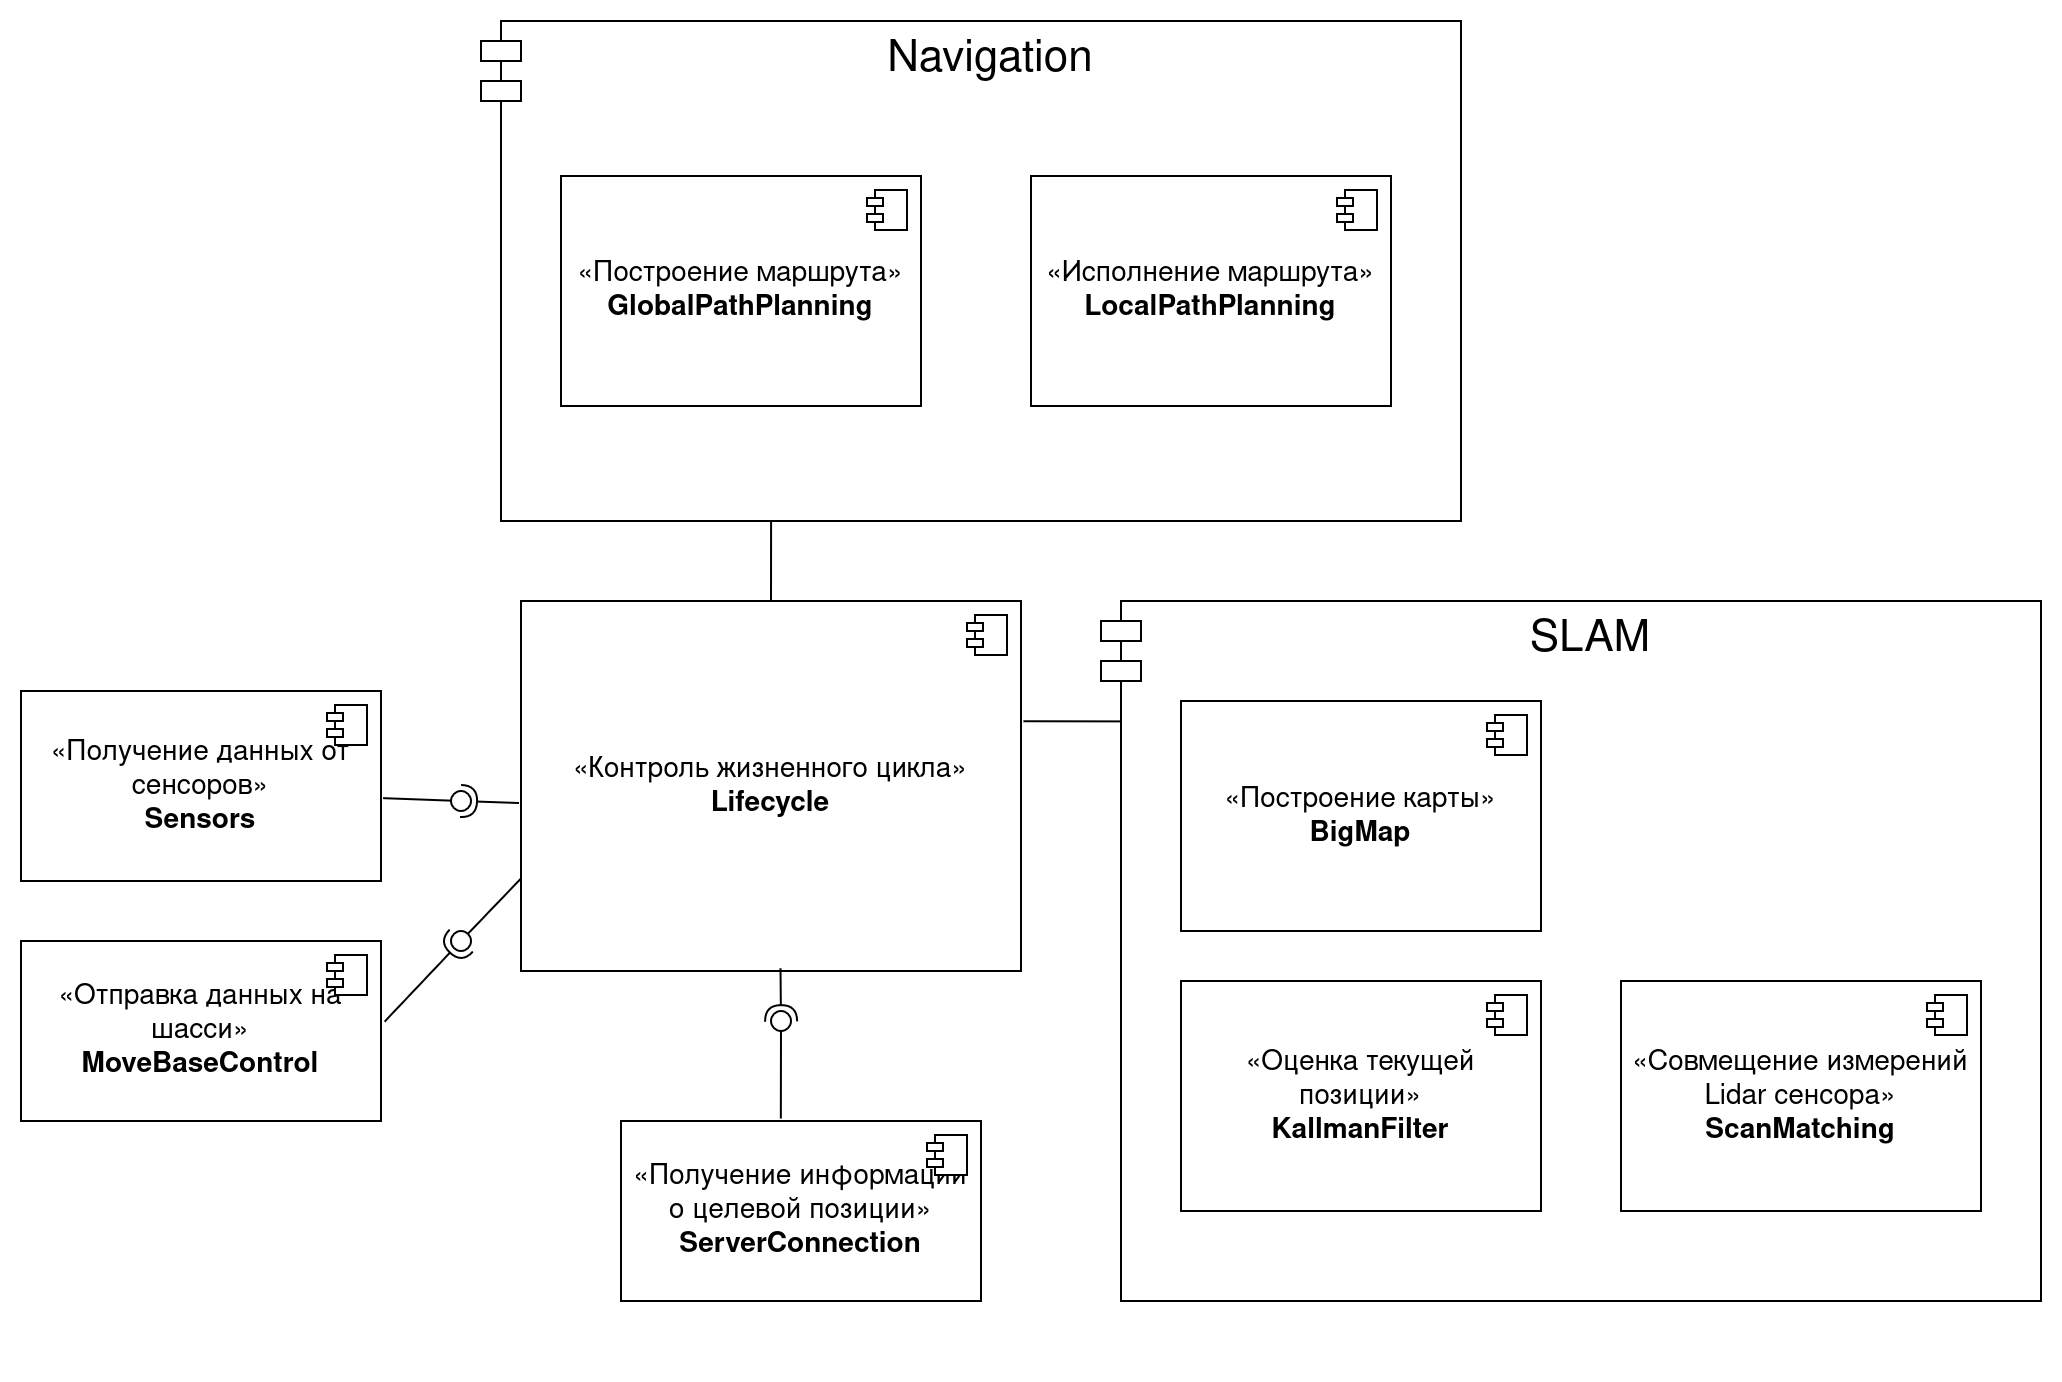
\includegraphics[width=11cm]{MODULES.drawio}}
\caption{Диаграмма компонентов проектируемого ПО}
\label{fig:components}
\end{figure}

На рисунке \ref{fig:components} отображены модули системы:~
\begin{itemize}
	\item модуль жизненного цикла;
	\item модуль построения маршрута;
	\item модуль исполнения маршрута;
	\item модуль получения данных сенсоров;
	\item модуль отправки данных на шасси;
	\item модуль получения информации о целевой позиции;
	\item модуль построения карты;
	\item модуль оценки позиции;
	\item модуль совмещения измерений Lidar сенсора.
\end{itemize}

% \todo{Общая схема программы}
Коммуникация между модулями осуществляется через модуль жизненного цикла, все
модули получают и отправляют информацию через него, не считая сильно-связных
модулей в системе SLAM. 

% Модули сбора информации
Модуль получения данных сенсоров осуществляет сбор информации: 2D Lidar
предоставляет информацию о расстояниях до объектов в окружающем пространстве,
IMU -- об угловых ускорениях и наклоне устройства, а GPS -- о
глобальном местоположении. Все эти данные передаются в модуль SLAM, который
использует их для построения карты окружающей среды и вычисления текущего
местоположения робота. Это позволяет системе иметь точную картину окружающего
мира и следить за положением устройства.

Модуль совмещения измерений Lidar сенсора, является основой для построения карты
и локализации робота. С помощью данных от лидаров и модуля оценки позиции он
строит карту пространства, постоянно обновляя ее по мере движения робота, и
вычисляет его местоположение относительно этой карты. Это позволяет системе
динамично корректировать действия робота в зависимости от изменений в окружающей
среде, таких как появление новых препятствий или изменение положения объектов.

Полученные от совмещения измерений данные о местоположении робота передаются в модуль оценки
позиции. Этот модуль анализирует текущее положение устройства с использованием
фильтрации и различных методов оценки, таких как фильтр Калмана. Оценка позиции
робота имеет важное значение для корректного планирования маршрута, поскольку
точность информации о местоположении напрямую влияет на точность движений
устройства.

Модуль создания маршрута отвечает за вычисление оптимального пути от текущего
местоположения робота до заданной цели. Этот модуль использует данные о
местоположении, а также информацию о препятствиях, чтобы планировать наиболее
эффективный и безопасный маршрут. Важно, чтобы система могла адаптироваться к
изменениям окружающей среды, например, при возникновении новых препятствий,
система должна пересчитать маршрут в реальном времени, обеспечивая продолжение
движения робота без ошибок.

После того как маршрут спланирован, информация о нем передается в модуль
управления моторами. Этот модуль отвечает за выполнение команд, таких как
движение вперед, повороты и торможение. Модуль управления моторами должен
обеспечить точное выполнение команд с минимальными задержками, чтобы робот мог
двигаться по маршруту с высокой точностью. Кроме того, он должен поддерживать
оперативную реакцию на данные от сенсоров, такие как сигнал от лидаров,
предупреждающий о близко расположенных препятствиях.

При обнаружении препятствий вблизи, например, если расстояние до объекта
становится меньше заданного порога, система должна немедленно реагировать. Это
может быть реализовано командой «стоп», которая отправляется в модуль управления
моторами для немедленной остановки робота. Такие меры безопасности необходимы
для предотвращения столкновений и обеспечения безопасной работы робота в
различных условиях.

\subsection{Модель состояния системы}

Для описания динамики системы используется вектор состояния \(X\):
\[
{X} = (x, y, v_x, v_y, a_x, a_y, \theta, v_\theta, a_\theta)^T,
\]

\begin{explanationx}
\item[где] $x, y$ -- координаты объекта в локальной карте, м;
\item $v_x, v_y$ -- компоненты скорости по осям $x$ и $y$, м/с;
\item $a_x, a_y$ -- компоненты ускорения по осям $x$ и $y$, м/с${}^2$;
\item $\theta$ -- угол ориентации объекта, $рад$;
\item $v_\theta$ -- угловая скорость, рад/с;
\item $a_\theta$ -- угловое ускорение, рад/с${}^2$.
\end{explanationx}

Выбор данной модели состояния обусловлен следующими факторами:
\begin{enumerate}[label=\arabic*]
    \item Вектор состояния включает положение, скорость и ускорение объекта как в поступательном, так и в угловом движении. 
	   Это позволяет точно описать сложные траектории, включая вращение.
    \item Включение ускорений ($a_x, a_y, a_\theta$), то есть использование модели константное ускорения,
	  позволяет моделировать изменения скорости и ориентации. Таким образом,
	повышается точность предсказания в условиях неравномерного движения.
\end{enumerate}

В данной системе с вектором состояния 
\({X} = (x, y, v_x, v_y, a_x, a_y, \theta, v_\theta, a_\theta)^T\)
используются линейная модель преобразования состояния (\(F\)) и линейная модель преобразования к измерениям (\(H\)).
Эти модели описывают динамику системы и связь состояния с измерениями от датчиков (GPS и LIDAR), соответственно.

\subsection{Модель преобразования состояния}
\label{subsec:state_transition}

Модель преобразования состояния описывает эволюцию вектора состояния \({X}_t\) во времени и задаётся линейным уравнением:
\[
{X}_{t+1} = {F} {X}_t + {w}_t.
\]
\begin{explanationx}
	\item[где] \({F}\) -- матрица перехода состояния, 
	\item \({w}_t \sim \mathcal{N}(0, {Q})\) -- гауссов шум процесса с ковариацией \({Q}\).
\end{explanationx}

Для вектора состояния \({X} = (x, y, v_x, v_y, a_x, a_y, \theta, v_\theta, a_\theta)^T\),
матрица \({F}\) имеет блочно-диагональную структуру,
отражая кинематические зависимости для поступательного и углового движения.
Пример структуры матрицы \({F}\) (для времени шага \(\Delta t\)) выглядит следующим образом:

\begin{equation}
{F} =
\begin{bmatrix}
1 & 0 & \Delta t & 0 & \frac{1}{2} \Delta t^2 & 0 & 0 & 0 & 0 \\
0 & 1 & 0 & \Delta t & 0 & \frac{1}{2} \Delta t^2 & 0 & 0 & 0 \\
0 & 0 & 1 & 0 & \Delta t & 0 & 0 & 0 & 0 \\
0 & 0 & 0 & 1 & 0 & \Delta t & 0 & 0 & 0 \\
0 & 0 & 0 & 0 & 1 & 0 & 0 & 0 & 0 \\
0 & 0 & 0 & 0 & 0 & 1 & 0 & 0 & 0 \\
0 & 0 & 0 & 0 & 0 & 0 & 1 & \Delta t & \frac{1}{2} \Delta t^2 \\
0 & 0 & 0 & 0 & 0 & 0 & 0 & 1 & \Delta t \\
0 & 0 & 0 & 0 & 0 & 0 & 0 & 0 & 1
\end{bmatrix}.
\end{equation}

Матрица F отражает линейную модель поступательного движения 
и модель углового движения:
\begin{equation}
\label{eq:state_transition_system}
\left\{
\begin{aligned}
x_{t+1} &= x_t + v_{x,t} \Delta t + \frac{1}{2} a_{x,t} \Delta t^2, \\
v_{x,t+1} &= v_{x,t} + a_{x,t} \Delta t, \\
a_{x,t+1} &= a_{x,t} + w_{a_x,t}, \\
y_{t+1} &= y_t + v_{y,t} \Delta t + \frac{1}{2} a_{y,t} \Delta t^2, \\
v_{y,t+1} &= v_{y,t} + a_{y,t} \Delta t, \\
a_{y,t+1} &= a_{y,t} + w_{a_y,t}, \\
\theta_{t+1} &= \theta_t + v_{\theta,t} \Delta t + \frac{1}{2} a_{\theta,t} \Delta t^2, \\
v_{\theta,t+1} &= v_{\theta,t} + a_{\theta,t} \Delta t, \\
a_{\theta,t+1} &= a_{\theta,t} + w_{a_\theta,t}.
\end{aligned}
\right.
\end{equation}

\subsection{Модель измерений}
\label{sec:measurement_model}

Модель измерений связывает вектор состояния \({X}_t\) с вектором измерений \({z}_t\):

\begin{equation}
{z}_t = {H} {X}_t + {v}_t,
\label{eq:measurement_model}
\end{equation}

\begin{explanationx}
	\item[где] \({H}\) -- матрица измерений,
	\item \({v}_t \sim \mathcal{N}(0, {R})\) -- гауссов шум измерений с ковариацией \({R}\).
\end{explanationx}

\subsubsection{Вектор измерений}
\label{subsec:measurement_vector}

Вектор измерений \({z}_t\) включает компоненты от GPS и LIDAR. Предполагается, что GPS предоставляет координаты \((x, y)\), а LIDAR -- координаты \((x, y)\) и угол ориентации \(\theta\). Таким образом, вектор измерений имеет вид:
\[
{z}_t = [x_{\text{GPS}}, y_{\text{GPS}}, x_{\text{LIDAR}}, y_{\text{LIDAR}}, \theta_{\text{LIDAR}}]^T.
\]
Размерность \({z}_t\) равна 5 (две координаты от GPS, две координаты и угол от LIDAR), 
хотя в случае асинхронного поступления данных некоторые компоненты могут быть недоступны в определённые моменты времени.

\subsubsection{Матрица измерений \({H}\)}
\label{subsec:measurement_matrix}

Матрица \({H}\) (см. уравнение \ref{eq:mes_transition}) размером \(5 \times 9\)
заполняется единицами только в позициях, соответствующих измеряемым компонентам состояния.
\begin{equation}
	\label{eq:mes_transition}
	{H} =
	\begin{bmatrix}
	1 & 0 & 0 & 0 & 0 & 0 & 0 & 0 & 0 \\
	0 & 1 & 0 & 0 & 0 & 0 & 0 & 0 & 0 \\
	1 & 0 & 0 & 0 & 0 & 0 & 0 & 0 & 0 \\
	0 & 1 & 0 & 0 & 0 & 0 & 0 & 0 & 0 \\
	0 & 0 & 0 & 0 & 0 & 0 & 1 & 0 & 0
	\end{bmatrix}.
\end{equation}

\subsubsection{Обработка асинхронных измерений}
\label{subsec:async_measurements}

В случае асинхронного поступления данных от GPS и LIDAR, если в момент времени \(t\) доступны 
не все компоненты \({z}_t\), 
матрица \({H}\) и вектор \({z}_t\) усекаются до соответствующих строк и элементов. 
Например, если доступны только данные GPS (\({z}_t = [x_{\text{GPS}}, y_{\text{GPS}}]^T\)), используется подматрица:
\[
{H}_{\text{GPS}} =
\begin{bmatrix}
1 & 0 & 0 & 0 & 0 & 0 & 0 & 0 & 0 \\
0 & 1 & 0 & 0 & 0 & 0 & 0 & 0 & 0
\end{bmatrix}.
\]
Аналогично, для данных от LIDAR (\({z}_t = [x_{\text{LIDAR}}, y_{\text{LIDAR}}, \theta_{\text{LIDAR}}]^T\)) используется:
\[
{H}_{\text{LIDAR}} =
\begin{bmatrix}
1 & 0 & 0 & 0 & 0 & 0 & 0 & 0 & 0 \\
0 & 1 & 0 & 0 & 0 & 0 & 0 & 0 & 0 \\
0 & 0 & 0 & 0 & 0 & 0 & 1 & 0 & 0
\end{bmatrix}.
\]
Ковариационная матрица шума \({R}\) также корректируется в зависимости от доступных измерений.


\subsubsection{Нелинейность модели}
\label{sec:ukf_choice}

Хотя модели преобразования состояния \({F}\) и измерений \({H}\) в данной системе линейны,
для оценки состояния был выбран UKF вместо линейного фильтра Калмана. Основная причина выбора UKF заключается в:
\begin{enumerate}[label=\arabic*]
	\item Необходимости корректной обработки угловой компоненты \(\theta\), 
		которая, несмотря на линейность модели, требует специального подхода к усреднению в циклическом пространстве углов.
		Например, через тригонометрические функции \(\sin\) и \(\cos\) для учёта переходов через \(0/2\pi\)).
	\item UKF обеспечивает повышенную устойчивость к выбросам в данных GPS и LIDAR, 
		эффективно обрабатывает асинхронные измерения благодаря очередям событий и обладает гибкостью для адаптации к
		возможным нелинейным расширениям модели в будущем.
\end{enumerate}

Алгоритм работы (UKF состоит из двух последовательных алгоритмов:
алгоритма шага предсказания (см. рисунок \ref{fig:ukf_predict}) 
и алгоритм шага обновления (см. рисунок \ref{fig:ukf_update}).

\FloatBarrier
\begin{figure}[H]
\centering
	\fbox{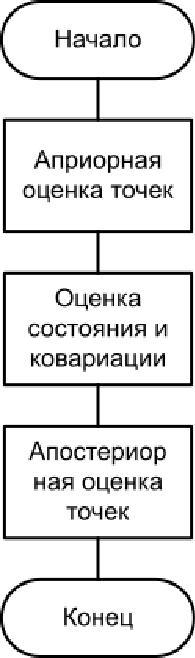
\includegraphics[height=10cm]{ukf_predict}}
\caption{Алгоритм шага предсказания UKF}
\label{fig:ukf_predict}
\end{figure}

На этапе предсказания UKF генерирует набор сигма-точек на основе текущей оценки состояния и ковариации, 
пропускает их через модель системы для прогнозирования следующего состояния и ковариации.
На этапе обновления, при поступлении измерений, сигма-точки пропускаются через модель измерений, после чего вычисляются среднее измерение, 
ковариация и коэффициент усиления Калмана, используемые для корректировки состояния и ковариации с учётом новых данных.
Этот подход позволяет UKF эффективно обрабатывать нелинейности и обеспечивать точную оценку состояния.

\FloatBarrier
\begin{figure}[H]
\centering
	\fbox{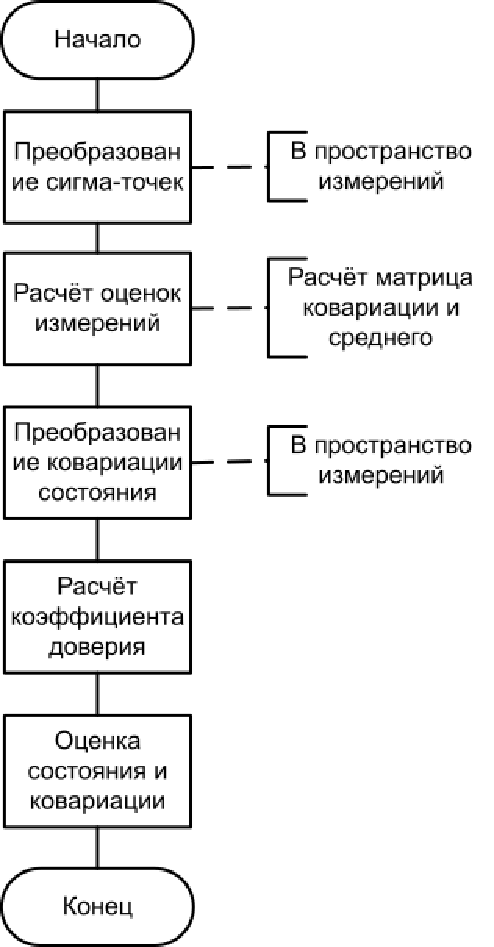
\includegraphics[height=12cm]{ukf_update}}
\caption{Алгоритм шага обновления UKF}
\label{fig:ukf_update}
\end{figure}

\subsubsection{События обновления состояния}

Данные от датчиков формируют события изменения состояния. 
Все события изменяют состояние системы в соответствии с алгоритмом обработки событий (см. рисунок \ref{fig:handle_kf_event})

\FloatBarrier
\begin{figure}[H]
\centering
	\fbox{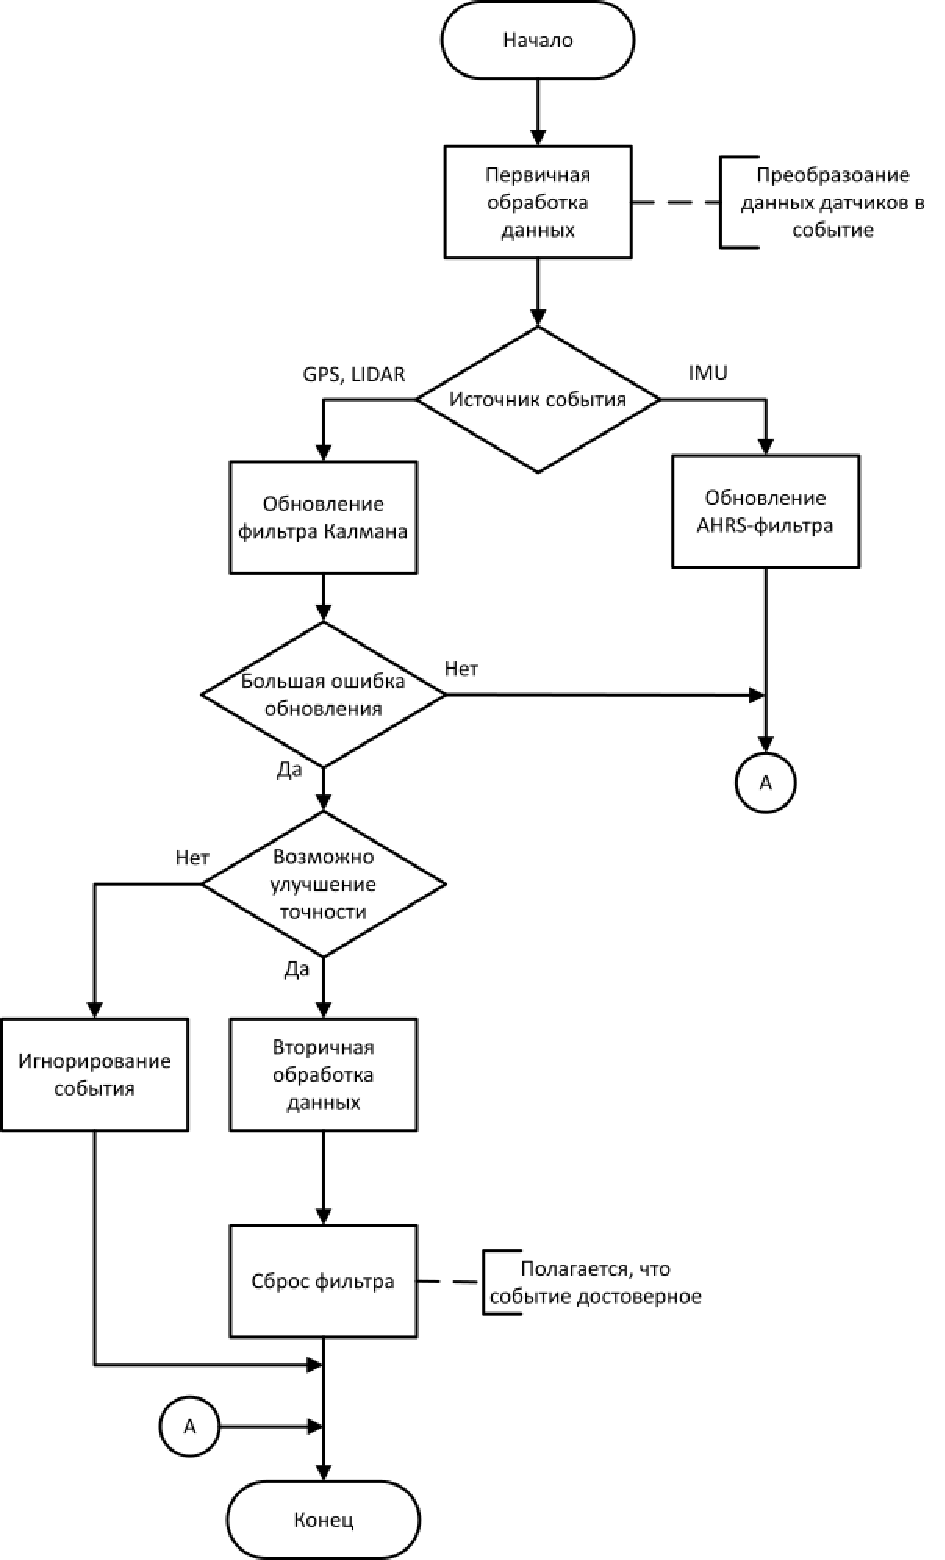
\includegraphics[height=12cm]{handle_event}}
\caption{Алгоритм обработки событий}
\label{fig:handle_kf_event}
\end{figure}


Обновление состояния в UKF выполняется только по позиционным событиям, 
которые происходят относительно редко, но обладают высокой точностью.
Позиционными событими являются содержат оценку координат робот в системе координат локальной карты робота ($x, y$) и
необязательную оценку ориентации робота в пространстве ($\theta$).
К таким событиям относятся результаты обработки данных от GPS и LIDAR.

Для обработки данных IMU используется фильтр Маджвика (см. подраздел \href{sec:ahrs}). Было принято решение использовать
отдельный фильтр для обработки данных IMU, а не обновлять вектор системы ${X}$,
по следующим причинам:
\begin{itemize}
	\item данные IMU измеряют только ориентацию, потому фильтр не сможет произвести коррекцию
	      всего вектора состояния во времени;
        \item данные от IMU приходят с гораздо большей частотой (1000 Hz), чем данные от LIDAR (10 Hz) или GPS (5 Hz).
\end{itemize}

Оценка ориентации с помощью фильтра Маджвика используется 
в процессе обработки данных LIDAR или GPS для формирования позиционных событий.

Таким образом, использованием фильтра Маджвика обеспечивает надежную и частую оценку ориентации, в то время как UKF использует редкие, но точные позиционные данные для коррекции полного вектора состояния.
Это повышает общую точность и устойчивость системы в условиях сложной динамики и возможных выбросов в измерениях.

\subsection{Очереди событий и очереди состояний}
\label{subsec:queues}

Каждое состояние системы ${X}_k$ и событие ${E}_k$ 
закреплено к моменту времени $t_k$. Каждое новое событие 
обновляет модель системы в сооветствие с алгоритмом применения события (см. рисунок \ref{fig:apply_kf_event})
\FloatBarrier
\begin{figure}[H]
\centering
	\fbox{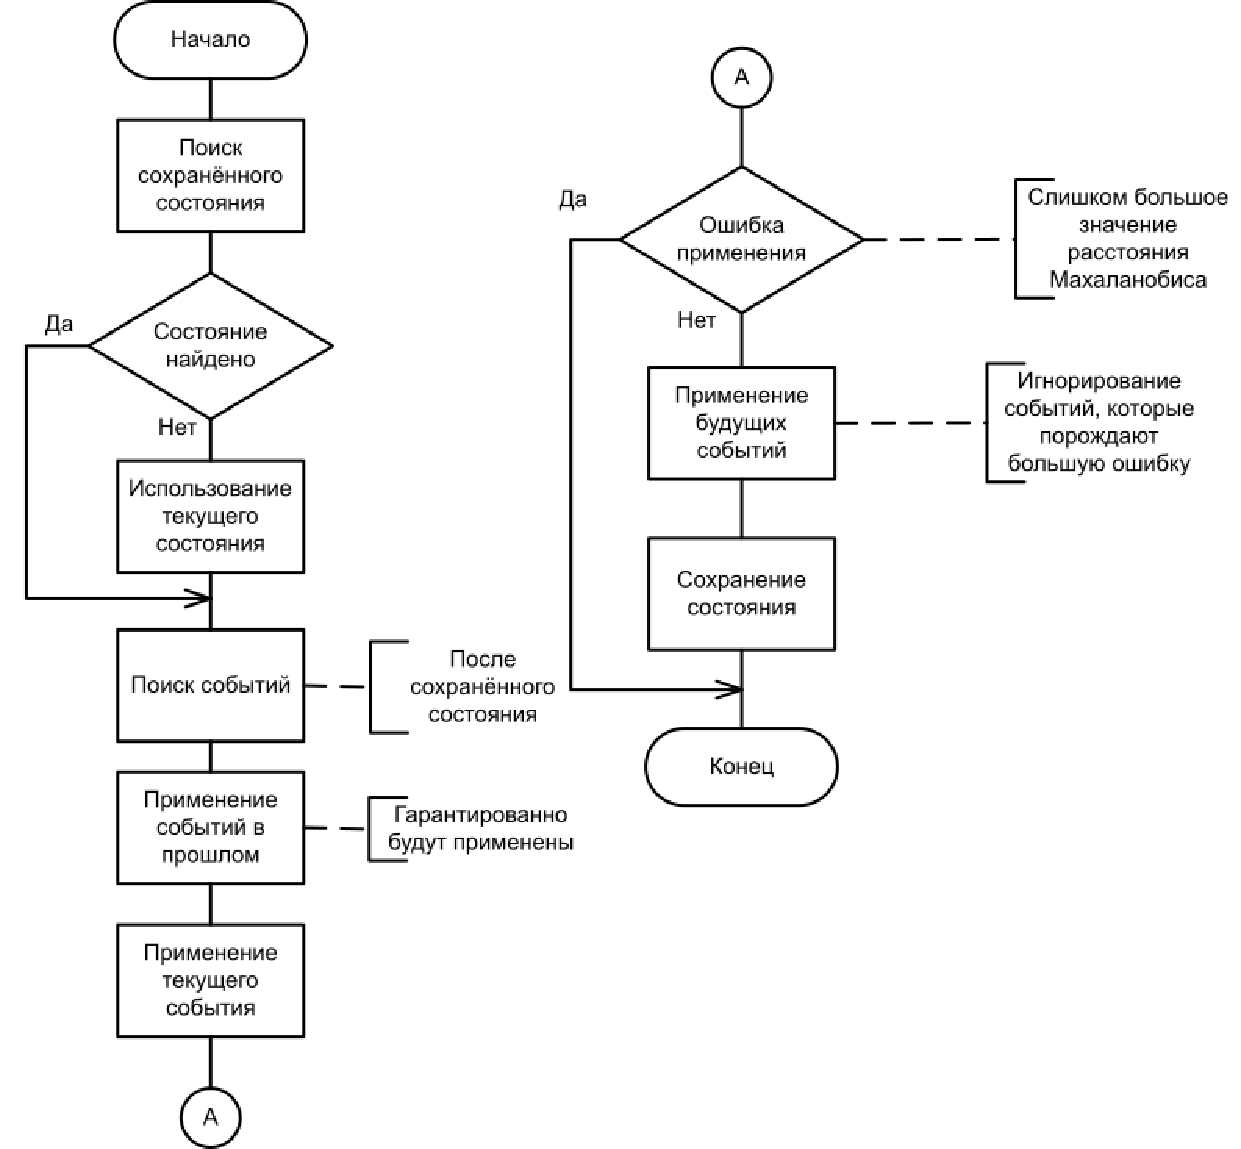
\includegraphics[height=12cm]{apply_event}}
\caption{Алгоритм применения события}
\label{fig:apply_kf_event}
\end{figure}

Для эффективной обработки данных и управления временной динамикой системы реализованы очереди состояний и событий.
Это позволяет синхронизировать данные от различных источников и корректно обновлять состояние системы в UKF.

\subsubsection{Очередь состояний}
\label{subsec:state_queue}

Очередь состояний представляет собой упорядоченный набор векторов состояния системы.
Основные характеристики очереди состояний:
\begin{itemize}
    \item каждое состояние в очереди соответствует определённому моменту времени, что позволяет отслеживать эволюцию системы и выполнять ретроспективные корректировки при получении новых данных;
    \item временные метки состояний используются для сопоставления с событиями, обеспечивая согласованность между предсказаниями и измерениями;
    \item при поступлении новых данных очередь состояний обновляется, добавляя новое состояние.
\end{itemize}

\subsubsection{Очередь событий}
\label{subsec:event_queue}

Очередь событий содержит результаты обработки данных от датчиков. Каждое из событие связано с моментом времени $t$.
События представляют собой позиционные данные, которые используются для коррекции состояния в UKF.
Основные характеристики очереди событий:
\begin{itemize}
    \item каждое событие имеет метку времени для определения положения относительно текущего момента времени;
    \item относительно события с временем $t_{\text{current}}$ события разделяются на события прошлого и события будущего;
    \item события прошлого используются для ретроспективной коррекции состояний, если данные поступили с задержкой или требуется уточнение предыдущих оценок;
    \item события будущего хранятся в очереди для обработки по мере продвижения текущего времени системы. Это позволяет системе быть готовой к асинхронным данных.
    \item очередь событий поддерживает асинхронное поступление данных от датчиков с разной частотой. 
\end{itemize}

\subsection{Планирование движения}

\subsubsection{Локальный планировщик}
В качестве локального планировщика используется DWA.
Целевая функция:
\begin{equation}
	G(v, \omega) = \sum_{i=1}^k w_i \cdot g_{i, \text{norm}}(v, \omega),
\end{equation}

\begin{explanationx}
	\item[где] $g_{i,\text{norm}}(v, \omega)$ -- значение $i$-й подцелевой функции;
	\item $w_i$ -- весовой коэффициент,
		настраиваемый для задания приоритетов;
	\item $k$ -- количество метрик.
\end{explanationx}

Для обеспечения сравнимости метрик,
имеющих разные единицы измерения и диапазоны,
значения подцелевых функций $g_i(v, \omega)$ нормализуются по всем возможным парам скоростей 
в динамическом окне $V_d$.
Нормализованное значение вычисляется как:
\begin{equation}
	g_{i, \text{norm}}(v, \omega) = \frac{g_i(v, \omega) - \min_{(v', \omega') \in V_d} g_i(v', \omega')}{\max_{(v', \omega') \in V_d} g_i(v', \omega') - \min_{(v', \omega') \in V_d} g_i(v', \omega')},
\end{equation}

\begin{explanationx}
	\item[где] $\min_{(v', \omega') \in V_d} g_i(v', \omega')$ --
минимальное значения $i$-й подцелевой функции среди всех пар $(v', \omega')$ в $V_d$.
	\item $\max_{(v', \omega') \in V_d} g_i(v', \omega')$ --
максимальное значения $i$-й подцелевой функции среди всех пар $(v', \omega')$ в $V_d$.
\end{explanationx}

Нормализация приводит значения к диапазону $[0, 1]$, что позволяет весам $w_i$ эффективно управлять
приоритетами метрик и обеспечивает сбалансированную оценку траекторий.

Для каждой пары скоростей предлагается построение уникальной траектории.
Оценка происходит не столько по значениями скорости, сколько по траекториям, которые скорости генерируют.
В качестве метрик предлагается использовать:

    1 Метрика близости к цели -- чем ближе конечная точка траектория к цели, тем траектория приоритетнее.

    2 Метрика близости к глобальной траектории -- чем ближе форма траектории к прямолинейной форме траектории, тем траектория приоритетнее.  

    3 Метрика избегания препятствий -- приоритет отдаётся тем траектории, которые проходят дальше от препятствий.

    4 Метрика колебательных движений -- предотвращает резкие (осциллирующие) изменения скоростей для обеспечения плавности и зацикливания.

    5 Выравнивание по целевой ориентаци -- инимизирует отклонение ориентации робота от желаемого угла в целевой точке.

    6 Метрика коллизий -- отклоняет все траектории, в которых обнаружены столкновения с объектами препятствий.

% \subsubsection{Применение}

% \subsubsection{Глобальный планировщик}

\subsection{Взаимодействие с периферией}


В процессе разработки программного обеспечения для автономной навигации
мобильных платформ одной из ключевых задач стало обеспечение гибкого и надёжного
взаимодействия с периферийными устройствами, такими как датчики, камеры и
лидары. После анализа различных подходов было принято решение реализовать это
взаимодействие с использованием стека протоколов TCP/IP. Такой выбор обусловлен
универсальностью и стандартизацией данного протокола, который широко применяется
в сетевых технологиях и позволяет организовать стабильное соединение между
компонентами системы. Это решение обеспечивает возможность передачи данных в
реальном времени, что критически важно для задач управления и обработки
информации в динамичной среде.

Использование TCP/IP стека предоставляет значительное преимущество в виде
модульности и расширяемости системы. Благодаря этому подходу стало возможным
подключение различных датчиков к программе непосредственно во время её работы,
без необходимости останавливать или перезапускать систему. Например, если в
процессе эксплуатации мобильной платформы потребуется добавить новый лидар или
ультразвуковой датчик, это можно сделать "на лету", что существенно повышает
адаптивность системы к изменяющимся условиям или требованиям задачи. Такая
гибкость особенно ценна в экспериментальных или полевых условиях, где заранее
предусмотреть все сценарии использования невозможно.

Реализация взаимодействия через TCP/IP также упрощает интеграцию с современными
технологиями и стандартами, используемыми в робототехнике. Например, многие
устройства уже имеют встроенную поддержку сетевых протоколов, что позволяет
избежать разработки сложных проприетарных интерфейсов для каждого типа
периферии. Кроме того, TCP/IP обеспечивает надёжную передачу данных с механизмом
проверки ошибок, что снижает риск потери критически важной информации от
датчиков. Это особенно актуально для автономных систем, где точность и
своевременность получения данных напрямую влияют на качество навигации и
принятия решений.

% \subsection{Разработка архитектуры модуля \todo{MotionEstimation}}
%
% \todo{Схема для motionEstimation}
%
% \subsection{Разработка архитектуры модуля \todo{BigMap}}
%
% \subsection{Разработка архитектуры модуля \todo{ScanMatching}}
%
% \subsection{Разработка архитектуры модуля \todo{TODO}}
